This calculator represents a decision-support tool for deciding whether the
employment of retrofitting measures to a collection of existing buildings is
advantageous from an economical point of view. For this assessment, the
expected losses considering the original and retrofitted configuration of the
buildings are estimated, and the economic benefit due to the better seismic
design is divided by the retrofitting cost, leading to the benefit/cost ratio.
These loss curves are computed using the previously described Classical PSHA-
based Risk calculator. The output of this calculator is a benefit/cost ratio
for each asset, in which a ratio above one indicates that employing a
retrofitting intervention is economically viable.

In Figure~\ref{fig:io-structure-benefit-cost}, the input/output structure for
this calculator is depicted.

\begin{figure}[ht]
\centering
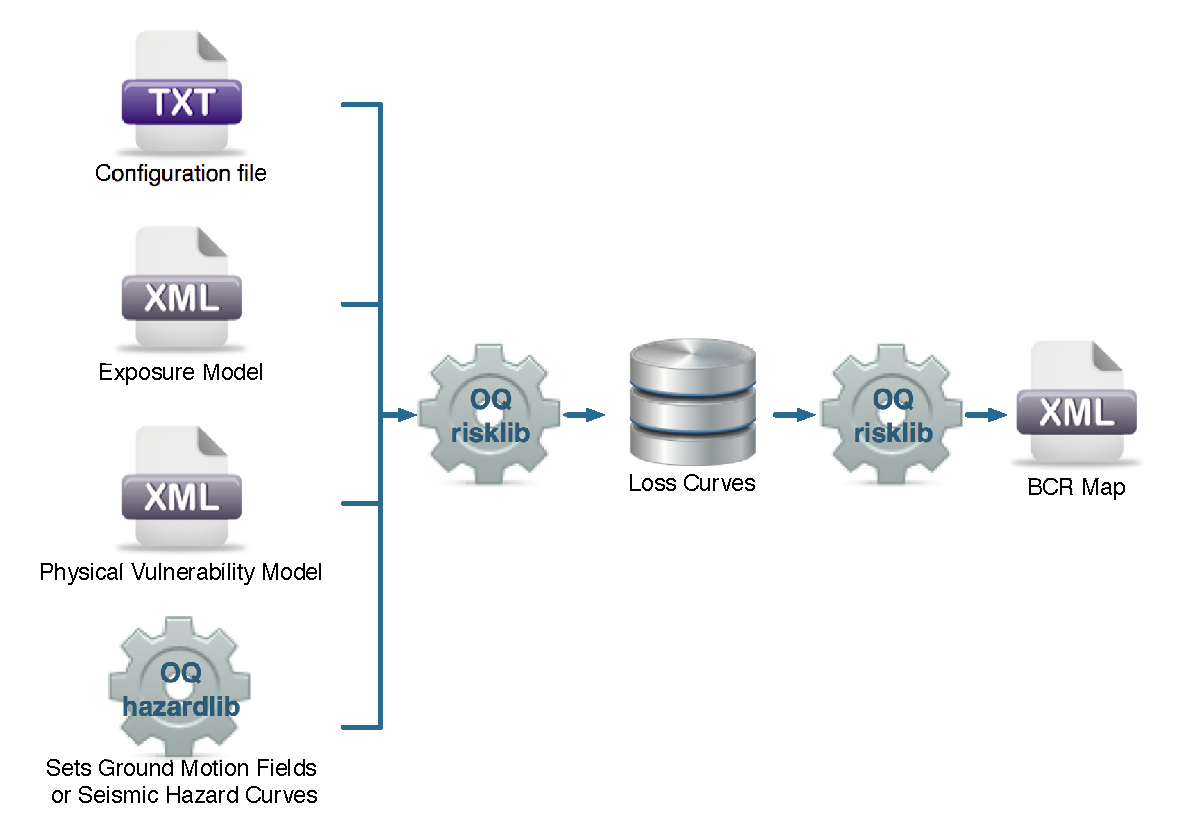
\includegraphics[width=10.5cm,height=7cm]{figures/risk/io-structure-benefit-cost.pdf}
\caption{Retrofitting Benefit/Cost Ratio Calculator input/output structure.}
\label{fig:io-structure-benefit-cost}
\end{figure}